\section*{Exercises}
 \addcontentsline{toc}{section}{Exercises}

\begin{excersizelist}

\item \label{eq:bandlimitedexampleforfir} Let $x$ be the signal with Fourier transform 
\[
\hat{x}(f) = \tfrac{4}{3}\rect(f) - \cos(2\pi f) \big( \rect(2f - 3) + \rect(2f + 3) \big).
\]
Plot the Fourier transform.  Find and plot $x$.
\begin{solution}
A plot of the Fourier transform is below.

{
\centering
  \def\sx{1.2}
  \def\sy{2.5}
  \def\P{0.25}
  \def\F{(1/\P)}
  \def\c{1}
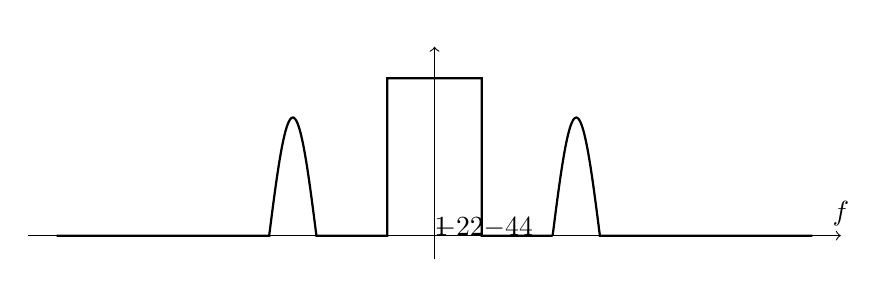
\begin{tikzpicture}
    \begin{scope}[yscale=\sy,xscale=\sx]
      
      % draw axis
      \draw[->] (-4.3,0) -- (4.3,0) node[above] {$f$};
      % \draw[->] (0,-0.35) -- (0,2.3) node[above,font=\footnotesize] {$\rect(f) \big(1 + \cos( 2 \pi f )\big) + \rect{3f - 2} + \rect{3f + 2}$};    
      \draw[->] (0,-0.2) -- (0,1.6) node[above,font=\footnotesize] {};  
      
      % draw unfiltered Fourier transform magnitude
       \draw[thick] (-4,0) -- (-1.75,0) 
       -- plot[smooth,domain=-1.75:-1.25,samples=50] (\x,{-cos(2*pi*\x r)})
       -- (-1.25,0) -- (-0.5,0) -- (-0.5,1.3333) -- (0.5,1.3333) -- (0.5,0) -- (1.25, 0)
       -- plot[smooth,domain=1.25:1.75,samples=50] (\x,{-cos(2*pi*\x r)})
       -- (1.75,0) -- (4,0);
      
      % add some axis ticks
    \end{scope}
    \begin{scope}[xscale=\sx]
      \vtick{-2.0} node[pos=0.5,below] {$-2$};
      \vtick{2} node[pos=0.5,below] {$2$};
      \vtick{-4.0} node[pos=0.5,below] {$-4$};
      \vtick{4} node[pos=0.5,below] {$4$};
    \end{scope}
    \begin{scope}[yscale=\sy]
      \htick{1} node[pos=0.5,above left] {$1$};
    \end{scope}
  \end{tikzpicture}
}

The time domain signal $x$ can be found by direct application of the inverse Fourier transform, but a simpler approach uses the time shifting, time scaling properties, and modulation properties of the Fourier transform (Section~\zref{sec:fourier-transform}).  Let $a$ be the signal with Fourier transform $\hat{a}(f) = \rect(2f)$.  The time scaling property asserts that
\[
a(t) = \tfrac{1}{2} \sinc\big(\tfrac{t}{2}\big).
\]
From the modulation property of the Fourier transform
\[
\calF\big( \cos(3\pi t)  a(t) \big) = \tfrac{1}{2} \hat{a}(f - \tfrac{3}{2}) + \tfrac{1}{2} \hat{a}(f + \tfrac{3}{2}) =  \tfrac{1}{2} \rect(2f - 3) + \tfrac{1}{2} \rect(2f +3)
\]
Let $b(t) = \cos(3\pi t)  a(t)$ so that $\hat{b}(f) = \tfrac{1}{2}\rect(2f - 3) + \tfrac{1}{2} \rect(2f +3)$.  Now, put 
\begin{align*}
c(t) &= T_{-1} b(t) + T_{1} b(t) \\
&= b(t+1) + b(t-1) \\
&= \cos(3\pi t + 3\pi)  a(t+1) + \cos(3\pi t - 3\pi)  a(t-1)
\end{align*}
and because 
\[
-\cos(3\pi t) = \cos(3\pi t + 3\pi) = \cos(3\pi t - 3\pi) 
\]
we have
\[
c(t) = -\cos(3\pi t)  \big( a(t+1) +  a(t-1) \big).
\]
From the time shift property of the Fourier transform
\begin{align*}
\hat{c}(f) &= \calF( T_{-1} b + T_{1} b ) \\
&= e^{2\pi f j } \hat{b}(f) + e^{-2\pi f j } \hat{b}(f) \\
&= 2\cos(2\pi f) \hat{b}(f) \\
&= \cos(2\pi f) \big( \rect(2f - 3) + \rect(2f + 3) \big).
\end{align*}
It remains to observe that
\[
\hat{x}(f) = \tfrac{4}{3}\rect(f) - \hat{c}(f)
\]
and so
\begin{align*}
x(t) &= \tfrac{4}{3} \sinc(f) - c(t) \\
&= \tfrac{4}{3} \sinc(f) + \cos(3\pi t)  \big( a(t+1) +  a(t-1) \big) \\
&= \tfrac{4}{3} \sinc(f) + \tfrac{1}{2} \cos(3\pi t) \left( \sinc\big(\tfrac{t+1}{2}\big) + \sinc\big(\tfrac{t-1}{2}\big) \right)
\end{align*}
This signal is plotted below.

{
\centering
  \def\sx{1.2}
  \def\sy{1.5}
  \def\P{0.25}
  \def\F{(1/\P)}
  \def\c{1}
  \def\sincf(#1){(sin(pi*(#1))/(pi*(#1)))} %sinc function
  \def\cfsig(#1){ 0.5*cos(3*pi*#1)*((\sincf(#1/0.5+0.5)) + (\sincf(#1/0.5-0.5))) }
  \def\xsig(#1){(4.0*\sincf(#1)/3.0) + \cfsig(#1)}
\begin{tikzpicture}
    \begin{scope}[yscale=\sy,xscale=\sx]
      
      % draw axis
      \draw[->] (-4.3,0) -- (4.3,0) node[above] {$f$};
      % \draw[->] (0,-0.35) -- (0,2.3) node[above,font=\footnotesize] {$\rect(f) \big(1 + \cos( 2 \pi f )\big) + \rect{3f - 2} + \rect{3f + 2}$};    
      \draw[->] (0,-0.2) -- (0,2.3) node[above,font=\footnotesize] {};  
      
      % draw time domain signal
       \draw[thick,smooth,domain=-4:4,samples=200] plot function{\xsig(x)};
%       \draw[thick,smooth,domain=-4:4,samples=100] plot function{\cfsig(x)};

      
      % add some axis ticks
    \end{scope}
    \begin{scope}[xscale=\sx]
      \vtick{-2.0} node[pos=0.5,below] {$-2$};
      \vtick{2} node[pos=0.5,below] {$2$};
      \vtick{-4.0} node[pos=0.5,below] {$-4$};
      \vtick{4} node[pos=0.5,below] {$4$};
    \end{scope}
    \begin{scope}[yscale=\sy]
      \htick{1} node[pos=0.5,above left] {$1$};
    \end{scope}
  \end{tikzpicture}
}


\end{solution}

\item \label{exer:blackmawindowfouriertransform} Find the Fourier transform of the Blackman window~\zeqref{eq:blackmanwindow}.

\item \label{exer:stepseqZtrans} Show that the z-transform of the sequence  $a^nu_n$ is $z/(z-a)$ with region of convergence $\abs{z} > \abs{a}$.
\begin{solution}
The z-transform is
\[
\calZ(a^nu_n) = \sum_{n \in \ints} a^n u_n z^{-n} = \sum_{n=0}^\infty \left(\frac{z}{a}\right)^{-n}.
\]
This sum is a geometric progression that converges to 
\[
\frac{1}{1- a z^{-1}} = \frac{z}{ z-a}
\]
when $\abs{z/a} > 1$ and diverges otherwise.  The region of convergence is thus $\abs{z} > \abs{a}$.
\end{solution}

\item \label{exer:fallingfacztransform} Show that the z-transform of the sequence $[n]_k u_n$ where $[n]_k = n(n-1)\dots(n-k+1)$ is a falling factorial is
\[
\calZ\big( [n]_k u_n  \big) = \frac{k! z }{(z - 1)^{k+1}} \qquad \abs{z} > 1.
\]
\begin{solution}
Observe that
\begin{align*}
\calZ\big( [n]_{k} u_n  \big) &= \sum_{n\in\ints} [n]_k u_n z^{-n} \\ 
&= \sum_{n=0}^\infty [n]_k z^{-n} \\ 
&= \sum_{n=-1}^\infty [n+1]_k z^{-(n+1)} \\
&= z^{-1} \sum_{n=-1}^\infty [n+1]_k z^{-n}.
\end{align*}
Because $[0]_k = 0 \times -1 \times \dots \times (1-k)= 0$ we have
\[
z \calZ\big( [n]_{k} u_n  \big) = \sum_{n=0}^\infty [n+1]_k z^{-n}.
\]  
Now
\begin{align*}
(z - 1) \calZ\big( [n]_{k} u_n  \big) &= \sum_{n=0}^\infty [n+1]_k z^{-n} - \sum_{n=0}^\infty [n]_k u_n z^{-n} \\
&= \sum_{n=0}^\infty ([n+1]_k - [n]_k) z^{-n}.
\end{align*}
Observe that the falling factorial satisfies
\begin{align*}
[n+1]_k - [n]_k &= \big( (n+1)n(n-1)\dots(n-k+2) \big) \;\;  - \;\; \big(n(n-1)\dots(n-k+1)\big) \\
&= [n]_{k-1}(n+1 - n+k-1) \\
&= [n]_{k-1} k
\end{align*}
and so
\begin{align*}
(z - 1) \calZ\big( [n]_{k} u_n  \big) &= k \sum_{n=0}^\infty  [n]_{k-1} z^{-n} \\
&= k \calZ\big( [n]_{k-1} u_n  \big).
\end{align*}
We obtain the following recursive equation for $\calZ\big( [n]_{k} u_n  \big)$,
\[
\calZ\big( [n]_{k} u_n  \big) = \frac{k}{z-1} \calZ\big( [n]_{k-1} u_n  \big).
\]
Unravelling this recursion we obtain
\[
\calZ\big( [n]_{k} u_n  \big) = \frac{k}{z-1} \times \frac{k-1}{z-1} \times \frac{k-2}{z-1} \times \dots \times \calZ( [n]_0 u_n ).
\]
By definition $[n]_0 = 1$ for all $n \in \ints$ and so $\calZ( [n]_0 u_n ) = \calZ( u_n ) = z/(z-1)$ with region of convergence $\abs{z} >1$.  Thus,
\[
\calZ\big( [n]_{k} u_n  \big) = \frac{k! z}{(z-1)^{k+1}} \qquad \abs{z} > 1
\]
as required.
\end{solution}

\item \label{exer:findimpulseresponsesecondorderdiscrete} Find the discrete impulse response of the discrete time system corresponding with the second order difference equation $c_n = d_n - a d_{n-1} - b d_{n-2}$. 

\item \label{exer:fftcomplexity} Let $d_n$ be a sequence satisfying $d_n = 2 d_{n-1} + 2^{n+1}$ and suppose that $d_0 = 0$.  Show that $d_n = 2^{n+1}n$ for $n = 1,2,\dots$.  %Find a similar expression for $d_n$ is the case that $d_0 = a \neq 0$.
\begin{solution}
In Section~\zref{sec:difference-equations} we found the discrete time system $H$ with discrete impulse response $h_n = 2^{n}u_n$ is such that the respone $y = Hx$ is input signal $x$ satisfied the equation
\[
x = y - 2 T_{P}(y).
\] 
Suppose that the sample period is $P=1$.  The response of $H$ to input signal is $x(t) = 2^{t+1}u(t)$ is
\begin{align*}
y = H(x) &= \sum_{n \in \ints} h_n T_{n}(x) \\
&= \sum_{n = 0}^\infty 2^n 2^{t-n+1}u(t-n) \\
&= 2^{t+1} \floor{t}u(t)
\end{align*}
Let $c$ and $d$ be sequences with elements 
\[
c_n = x(nP) = 2^{n+1}u_{n-1}, \qquad d_n = y(nP) = 2^{n+1}n u_n
\]
and observe that $d_0 = 0$.  By definition of $H$ these sequences satisfy the difference equation
\[
c_n = 2^{n+1}u_n = d_n - 2 d_{n-1}
\]
as required.

Let us now consider an alternative method of solution that applyies the z-transform directly to the difference equation
\[
 d_n - 2 d_{n-1} = 2^{n+1} u_{n-1}.
\]
Applying the z-transform to both sides and using the time shift property we have
\[
\calZ(d) - 2 z^{-1} \calZ(d) = \calZ(2^{n+1} u_n) = \frac{4}{z-2} \qquad \abs{z} > 2.
\]
The z-transform of $d$ is then
\[
\calZ(d) = \frac{4z}{(z-2)^2} \qquad \abs{z} > 2.
\]
The inverse z-transform is found by putting $k=1$ and $a = 2$ in~\zeqref{eeq:onlyztrans}.  We obtain $d_n = 2^{n+1} n u_n$.  Observing that $d_n = 0$ we have a solution.
\end{solution}

\item \label{exer:fibonacci} The Fibonacci sequence $0,1,1,2,3,5,8,13,\dots$ satisfies the recursive equation $d_0 = 0, d_1 = 1$, and $d_n = d_{n-1} + d_{n-2}$ for $n \geq 2$.  Find a closed form expression for the $n$th Fibonacci number.
\begin{solution}
Consider the recursive equation
\[
d_n - d_{n-1} - d_{n-2} = \delta_{n}.
\]
Applying z-transforms to both sides gives
\[
\calZ(d) - z^{-1} \calZ(d) - z^{-2} \calZ(d) = \calZ(\delta) = 1.
\]
The region of convergence is the whole complex plane.  We have
\[
\calZ(d) = \frac{z^2}{z^2 - z - 1} = z \left( \frac{z}{z^2 - z - 1} \right)
\]
Our formula for the inverse z-transformation~\zeqref{eeq:onlyztrans} involves $z$ on the numerator and so applying partial fractions to the term within the brackets will be convenient.  The roots of $z^2 - z - 1$ are
\[
a = \frac{1-\sqrt{5}}{2}, \qquad b = \frac{1+\sqrt{5}}{2}
\]
and by partial fractions (see Exercise~\ref{exer:partialfracsecondorder}) we obtain.
\[
\frac{z}{(z-a)(z-b)} = \frac{a}{(a-b) (z-a)}-\frac{b}{(a-b) (z-b)}
\]
and so
\[
\calZ(d) = \frac{az}{(a-b) (z-a)}-\frac{bz}{(a-b) (z-b)}
\]
Both of these terms are in the form of~\zeqref{eeq:onlyztrans} when $k=0$ and so
\[
d_n = \frac{1}{a-b} a^n u_n + \frac{1}{b-a} b^n u_n = \frac{b^n - a^n}{\sqrt{5}} u_n
\]
Observe that $d_0 = 0$ and that $d_1 = 1$ as a result of $b - a = 1$.
\end{solution}

% \item \label{excer:sumsqreexp} Show that $\sum_{n \in \ints} e^{a n^2} = ?$ if $a < 0$ (Hint: solve Excersize~\ref{excer:sumgeomeabsn} first).
% \begin{solution}
% BLERG: 
% \end{solution}

\begin{hardexercise}

\item \label{excer:stableimpulserespdiscretetime} Show that a discrete time system is stable if and only if its discrete impulse response is absolutely summable. 

% \item \label{exer:findtransfuncdiffeq} Suppose that $H$ is a linear time invariant system such that the response $y = H(x)$ to input $x$ satisfies~\zeqref{eq:differenceequformsystem}.  Find the transfer function of $H$.
% \begin{solution}
% Substitute $e^{st}$ for $x$ and $\lambda e^{st}$ for $y$ into~\zeqref{eq:differenceequformsystem},
% \begin{align*}
% \sum_{\ell=0}^{m} a_\ell T_{P\ell}(e^{st}) &= \sum_{\ell=0}^{k} b_\ell T_{P\ell}(\lambda e^{st}) \\
% \sum_{\ell=0}^{m} a_\ell e^{s(t-P\ell)} &= \sum_{\ell=0}^{k} b_\ell \lambda e^{s(t-P\ell)} \\
% \sum_{\ell=0}^{m} a_\ell e^{-sP\ell} &= \lambda \sum_{\ell=0}^{k} b_\ell e^{-sP\ell}.
% \end{align*}
% Solving for $\lambda$ yeilds the transfer function of $H$,
% \[
% \lambda(H,s) = \frac{\sum_{\ell=0}^{m} a_\ell e^{-sP\ell}}{\sum_{\ell=0}^{k} b_\ell e^{-sP\ell}}.
% \]
% \end{solution}

\item \label{exer:convabssummableisabssummable}  Let $f$ and $g$ be absolutely summable sequences.  Show that the discrete convolution $f * g$ is also absolutely summable.  


\item \label{exer:roczabssummrel} Let $H$ be a discrete time system with discrete impulse response $h$.  The set $\roc_z h$ is defined as those complex numbers $z = e^{sP}$ such that $s = \cep \dom_P h$.  Show that $\roc_z h$ is precisely the set of nonzero complex numbers such that the sequence $h_n z^{-n}$ is absolutely summable.


\item \label{excer:discrconvassociative} Let $f,g,h$ be complex valued sequences such that 
\[
\sum_{m \in \ints} \sum_{k \in \ints} \abs{f_{k} h_m g_{n-m-k}} < \infty.
\]
Show that the discrete convolution is associative for these sequences.  That is, show that $(f*g)*h = f*(g*h)$.
\begin{solution}
Let $f,g,h$ be sequences.  We have
\begin{align*}
((f*g)*h)_n &= \sum_{m \in \ints} h_{m} (f*g)_{n-m} \\
&= \sum_{m \in \ints} h_{m} \sum_{k \in \ints} g_{k} f_{n-m-k} \\
&= \sum_{m \in \ints} h_{m} \sum_{k \in \ints} f_{k} g_{n-m-k} \qquad \text{commutivity $f*g=g*f$} \\
&= \sum_{m \in \ints} \sum_{k \in \ints} f_{k} h_m g_{n-m-k} \\
\end{align*}
Under the assumptions stated on $f,g,h$ Fubini's theorem~\cite[Theorem~8.8]{Rudin_real_and_complex_analysis} may be used to justify swapping the order of summation leading to
\begin{align*}
((f*g)*h)_n &= \sum_{k \in \ints} \sum_{m \in \ints}  f_{k} h_m g_{n-k-m} \\
&= \sum_{k \in \ints} f_{k} \sum_{m \in \ints}  h_m g_{n-k-m} \\
&= \sum_{k \in \ints} f_{k} (g*h)_{n-k} \\
&= (f*(g*h))_n.
\end{align*}
\end{solution}

\end{hardexercise}

\end{excersizelist}




%%% Local Variables: 
%%% mode: latex
%%% TeX-master: "main.tex"
%%% End: 
